\documentclass[twoside]{book}

% Packages required by doxygen
\usepackage{fixltx2e}
\usepackage{calc}
\usepackage{doxygen}
\usepackage[export]{adjustbox} % also loads graphicx
\usepackage{graphicx}
\usepackage[utf8]{inputenc}
\usepackage{makeidx}
\usepackage{multicol}
\usepackage{multirow}
\PassOptionsToPackage{warn}{textcomp}
\usepackage{textcomp}
\usepackage[nointegrals]{wasysym}
\usepackage[table]{xcolor}

% Font selection
\usepackage[T1]{fontenc}
\usepackage[scaled=.90]{helvet}
\usepackage{courier}
\usepackage{amssymb}
\usepackage{sectsty}
\renewcommand{\familydefault}{\sfdefault}
\allsectionsfont{%
  \fontseries{bc}\selectfont%
  \color{darkgray}%
}
\renewcommand{\DoxyLabelFont}{%
  \fontseries{bc}\selectfont%
  \color{darkgray}%
}
\newcommand{\+}{\discretionary{\mbox{\scriptsize$\hookleftarrow$}}{}{}}

% Page & text layout
\usepackage{geometry}
\geometry{%
  a4paper,%
  top=2.5cm,%
  bottom=2.5cm,%
  left=2.5cm,%
  right=2.5cm%
}
\tolerance=750
\hfuzz=15pt
\hbadness=750
\setlength{\emergencystretch}{15pt}
\setlength{\parindent}{0cm}
\setlength{\parskip}{3ex plus 2ex minus 2ex}
\makeatletter
\renewcommand{\paragraph}{%
  \@startsection{paragraph}{4}{0ex}{-1.0ex}{1.0ex}{%
    \normalfont\normalsize\bfseries\SS@parafont%
  }%
}
\renewcommand{\subparagraph}{%
  \@startsection{subparagraph}{5}{0ex}{-1.0ex}{1.0ex}{%
    \normalfont\normalsize\bfseries\SS@subparafont%
  }%
}
\makeatother

% Headers & footers
\usepackage{fancyhdr}
\pagestyle{fancyplain}
\fancyhead[LE]{\fancyplain{}{\bfseries\thepage}}
\fancyhead[CE]{\fancyplain{}{}}
\fancyhead[RE]{\fancyplain{}{\bfseries\leftmark}}
\fancyhead[LO]{\fancyplain{}{\bfseries\rightmark}}
\fancyhead[CO]{\fancyplain{}{}}
\fancyhead[RO]{\fancyplain{}{\bfseries\thepage}}
\fancyfoot[LE]{\fancyplain{}{}}
\fancyfoot[CE]{\fancyplain{}{}}
\fancyfoot[RE]{\fancyplain{}{\bfseries\scriptsize Generated by Doxygen }}
\fancyfoot[LO]{\fancyplain{}{\bfseries\scriptsize Generated by Doxygen }}
\fancyfoot[CO]{\fancyplain{}{}}
\fancyfoot[RO]{\fancyplain{}{}}
\renewcommand{\footrulewidth}{0.4pt}
\renewcommand{\chaptermark}[1]{%
  \markboth{#1}{}%
}
\renewcommand{\sectionmark}[1]{%
  \markright{\thesection\ #1}%
}

% Indices & bibliography
\usepackage{natbib}
\usepackage[titles]{tocloft}
\setcounter{tocdepth}{3}
\setcounter{secnumdepth}{5}
\makeindex

% Hyperlinks (required, but should be loaded last)
\usepackage{ifpdf}
\ifpdf
  \usepackage[pdftex,pagebackref=true]{hyperref}
\else
  \usepackage[ps2pdf,pagebackref=true]{hyperref}
\fi
\hypersetup{%
  colorlinks=true,%
  linkcolor=blue,%
  citecolor=blue,%
  unicode%
}

% Custom commands
\newcommand{\clearemptydoublepage}{%
  \newpage{\pagestyle{empty}\cleardoublepage}%
}

\usepackage{caption}
\captionsetup{labelsep=space,justification=centering,font={bf},singlelinecheck=off,skip=4pt,position=top}

%===== C O N T E N T S =====

\begin{document}

% Titlepage & ToC
\hypersetup{pageanchor=false,
             bookmarksnumbered=true,
             pdfencoding=unicode
            }
\pagenumbering{roman}
\begin{titlepage}
\vspace*{7cm}
\begin{center}%
{\Large My Project }\\
\vspace*{1cm}
{\large Generated by Doxygen 1.8.11}\\
\end{center}
\end{titlepage}
\clearemptydoublepage
\tableofcontents
\clearemptydoublepage
\pagenumbering{arabic}
\hypersetup{pageanchor=true}

%--- Begin generated contents ---
\chapter{Class Index}
\section{Class List}
Here are the classes, structs, unions and interfaces with brief descriptions\+:\begin{DoxyCompactList}
\item\contentsline{section}{\hyperlink{structnode}{node} }{\pageref{structnode}}{}
\item\contentsline{section}{\hyperlink{structnode1}{node1} }{\pageref{structnode1}}{}
\item\contentsline{section}{\hyperlink{structnode__info}{node\+\_\+info} }{\pageref{structnode__info}}{}
\end{DoxyCompactList}

\chapter{File Index}
\section{File List}
Here is a list of all files with brief descriptions\+:\begin{DoxyCompactList}
\item\contentsline{section}{\hyperlink{Lab1_8c}{Lab1.\+c} }{\pageref{Lab1_8c}}{}
\end{DoxyCompactList}

\chapter{Class Documentation}
\hypertarget{classLeftistHeap}{}\section{Leftist\+Heap Class Reference}
\label{classLeftistHeap}\index{Leftist\+Heap@{Leftist\+Heap}}


Collaboration diagram for Leftist\+Heap\+:
\nopagebreak
\begin{figure}[H]
\begin{center}
\leavevmode
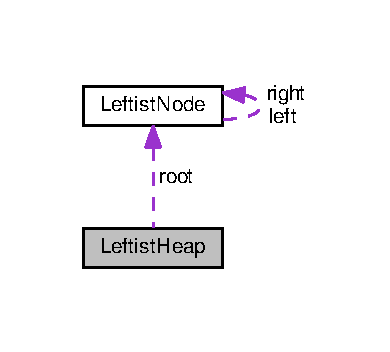
\includegraphics[width=187pt]{classLeftistHeap__coll__graph}
\end{center}
\end{figure}
\subsection*{Public Member Functions}
\begin{DoxyCompactItemize}
\item 
\hyperlink{classLeftistHeap_a07c9271159d856c743710e9eeabe10cb}{Leftist\+Heap} ()
\item 
\hyperlink{classLeftistHeap_a6ba1087bc57eaa696503673a8e0033da}{Leftist\+Heap} (\hyperlink{classLeftistHeap}{Leftist\+Heap} \&rhs)
\item 
\hyperlink{classLeftistHeap_a8476d82cfefc6b5557fa8242d34d61da}{$\sim$\+Leftist\+Heap} ()
\item 
bool \hyperlink{classLeftistHeap_a107b474e1c9f2a15710842d778305ca4}{is\+Empty} ()
\item 
bool \hyperlink{classLeftistHeap_a4ffa785d22e19ea689708ef68087724a}{is\+Full} ()
\item 
int \& \hyperlink{classLeftistHeap_aa04575171cef4ed3e1aeef7d2e7be1dd}{find\+Min} ()
\item 
void \hyperlink{classLeftistHeap_a1864cb85655de68ab0813579bd9b9659}{Insert} (int \&x)
\item 
void \hyperlink{classLeftistHeap_a41ab51a043541d4372fe10cd06561028}{delete\+Min} ()
\item 
void \hyperlink{classLeftistHeap_a6eed9075a7126edf3225498c8847aecd}{delete\+Min} (int \&min\+Item)
\item 
void \hyperlink{classLeftistHeap_a2032c8fd74f453ed323c43e016f40725}{make\+Empty} ()
\item 
void \hyperlink{classLeftistHeap_a30c5065cf2bd8c1816d944576f704cc7}{Merge} (\hyperlink{classLeftistHeap}{Leftist\+Heap} \&rhs)
\item 
\hyperlink{classLeftistHeap}{Leftist\+Heap} \& \hyperlink{classLeftistHeap_abc17697e82cfbf619ca15d0ca81cb415}{operator=} (\hyperlink{classLeftistHeap}{Leftist\+Heap} \&rhs)
\end{DoxyCompactItemize}
\subsection*{Private Member Functions}
\begin{DoxyCompactItemize}
\item 
\hyperlink{classLeftistNode}{Leftist\+Node} $\ast$ \hyperlink{classLeftistHeap_a89e92b6ef573c258f9e66fb37ffa10cc}{Merge} (\hyperlink{classLeftistNode}{Leftist\+Node} $\ast$h1, \hyperlink{classLeftistNode}{Leftist\+Node} $\ast$h2)
\item 
\hyperlink{classLeftistNode}{Leftist\+Node} $\ast$ \hyperlink{classLeftistHeap_a6cdfd2a56ec51b75bfe8cd870042ac6e}{Merge1} (\hyperlink{classLeftistNode}{Leftist\+Node} $\ast$h1, \hyperlink{classLeftistNode}{Leftist\+Node} $\ast$h2)
\item 
void \hyperlink{classLeftistHeap_a963d309aa88bea939ca56884f3b35110}{swap\+Children} (\hyperlink{classLeftistNode}{Leftist\+Node} $\ast$t)
\item 
void \hyperlink{classLeftistHeap_ac5a1f3154856b10909c77dff5f695273}{reclaim\+Memory} (\hyperlink{classLeftistNode}{Leftist\+Node} $\ast$t)
\item 
\hyperlink{classLeftistNode}{Leftist\+Node} $\ast$ \hyperlink{classLeftistHeap_aa2107259a308c39b8e147ecba2b1e888}{clone} (\hyperlink{classLeftistNode}{Leftist\+Node} $\ast$t)
\end{DoxyCompactItemize}
\subsection*{Private Attributes}
\begin{DoxyCompactItemize}
\item 
\hyperlink{classLeftistNode}{Leftist\+Node} $\ast$ \hyperlink{classLeftistHeap_a3c433b97cfbb2383f1fc75575df9005d}{root}
\end{DoxyCompactItemize}


\subsection{Constructor \& Destructor Documentation}
\index{Leftist\+Heap@{Leftist\+Heap}!Leftist\+Heap@{Leftist\+Heap}}
\index{Leftist\+Heap@{Leftist\+Heap}!Leftist\+Heap@{Leftist\+Heap}}
\subsubsection[{\texorpdfstring{Leftist\+Heap()}{LeftistHeap()}}]{\setlength{\rightskip}{0pt plus 5cm}Leftist\+Heap\+::\+Leftist\+Heap (
\begin{DoxyParamCaption}
{}
\end{DoxyParamCaption}
)}\hypertarget{classLeftistHeap_a07c9271159d856c743710e9eeabe10cb}{}\label{classLeftistHeap_a07c9271159d856c743710e9eeabe10cb}

\begin{DoxyCode}
58 \{
59     \hyperlink{classLeftistHeap_a3c433b97cfbb2383f1fc75575df9005d}{root} = NULL;
60 \}
\end{DoxyCode}
\index{Leftist\+Heap@{Leftist\+Heap}!Leftist\+Heap@{Leftist\+Heap}}
\index{Leftist\+Heap@{Leftist\+Heap}!Leftist\+Heap@{Leftist\+Heap}}
\subsubsection[{\texorpdfstring{Leftist\+Heap(\+Leftist\+Heap \&rhs)}{LeftistHeap(LeftistHeap &rhs)}}]{\setlength{\rightskip}{0pt plus 5cm}Leftist\+Heap\+::\+Leftist\+Heap (
\begin{DoxyParamCaption}
\item[{{\bf Leftist\+Heap} \&}]{rhs}
\end{DoxyParamCaption}
)}\hypertarget{classLeftistHeap_a6ba1087bc57eaa696503673a8e0033da}{}\label{classLeftistHeap_a6ba1087bc57eaa696503673a8e0033da}

\begin{DoxyCode}
66 \{
67     \hyperlink{classLeftistHeap_a3c433b97cfbb2383f1fc75575df9005d}{root} = NULL;
68     *\textcolor{keyword}{this} = rhs;
69 \}
\end{DoxyCode}
\index{Leftist\+Heap@{Leftist\+Heap}!````~Leftist\+Heap@{$\sim$\+Leftist\+Heap}}
\index{````~Leftist\+Heap@{$\sim$\+Leftist\+Heap}!Leftist\+Heap@{Leftist\+Heap}}
\subsubsection[{\texorpdfstring{$\sim$\+Leftist\+Heap()}{~LeftistHeap()}}]{\setlength{\rightskip}{0pt plus 5cm}Leftist\+Heap\+::$\sim$\+Leftist\+Heap (
\begin{DoxyParamCaption}
{}
\end{DoxyParamCaption}
)}\hypertarget{classLeftistHeap_a8476d82cfefc6b5557fa8242d34d61da}{}\label{classLeftistHeap_a8476d82cfefc6b5557fa8242d34d61da}

\begin{DoxyCode}
75 \{
76     \hyperlink{classLeftistHeap_a2032c8fd74f453ed323c43e016f40725}{makeEmpty}( );
77 \}
\end{DoxyCode}


\subsection{Member Function Documentation}
\index{Leftist\+Heap@{Leftist\+Heap}!clone@{clone}}
\index{clone@{clone}!Leftist\+Heap@{Leftist\+Heap}}
\subsubsection[{\texorpdfstring{clone(\+Leftist\+Node $\ast$t)}{clone(LeftistNode *t)}}]{\setlength{\rightskip}{0pt plus 5cm}{\bf Leftist\+Node} $\ast$ Leftist\+Heap\+::clone (
\begin{DoxyParamCaption}
\item[{{\bf Leftist\+Node} $\ast$}]{t}
\end{DoxyParamCaption}
)\hspace{0.3cm}{\ttfamily [private]}}\hypertarget{classLeftistHeap_aa2107259a308c39b8e147ecba2b1e888}{}\label{classLeftistHeap_aa2107259a308c39b8e147ecba2b1e888}

\begin{DoxyCode}
235 \{
236     \textcolor{keywordflow}{if} (t == NULL)
237         \textcolor{keywordflow}{return} NULL;
238     \textcolor{keywordflow}{else}
239         \textcolor{keywordflow}{return} \textcolor{keyword}{new} \hyperlink{classLeftistNode}{LeftistNode}(t->\hyperlink{classLeftistNode_a39afeded6425dbd13bbfd1d9fffb8a95}{element}, \hyperlink{classLeftistHeap_aa2107259a308c39b8e147ecba2b1e888}{clone}(t->\hyperlink{classLeftistNode_a62469c988fc0537dd6682d56f2108d99}{left}), 
      \hyperlink{classLeftistHeap_aa2107259a308c39b8e147ecba2b1e888}{clone}(t->\hyperlink{classLeftistNode_aee2ba46112890733b87007103122fc2a}{right}), t->\hyperlink{classLeftistNode_afcd068d744065dc1201d1f738b923447}{npl});
240 \}
\end{DoxyCode}
\index{Leftist\+Heap@{Leftist\+Heap}!delete\+Min@{delete\+Min}}
\index{delete\+Min@{delete\+Min}!Leftist\+Heap@{Leftist\+Heap}}
\subsubsection[{\texorpdfstring{delete\+Min()}{deleteMin()}}]{\setlength{\rightskip}{0pt plus 5cm}void Leftist\+Heap\+::delete\+Min (
\begin{DoxyParamCaption}
{}
\end{DoxyParamCaption}
)}\hypertarget{classLeftistHeap_a41ab51a043541d4372fe10cd06561028}{}\label{classLeftistHeap_a41ab51a043541d4372fe10cd06561028}

\begin{DoxyCode}
157 \{
158     \hyperlink{classLeftistNode}{LeftistNode} *oldRoot = \hyperlink{classLeftistHeap_a3c433b97cfbb2383f1fc75575df9005d}{root};
159     \hyperlink{classLeftistHeap_a3c433b97cfbb2383f1fc75575df9005d}{root} = \hyperlink{classLeftistHeap_a30c5065cf2bd8c1816d944576f704cc7}{Merge}(\hyperlink{classLeftistHeap_a3c433b97cfbb2383f1fc75575df9005d}{root}->\hyperlink{classLeftistNode_a62469c988fc0537dd6682d56f2108d99}{left}, \hyperlink{classLeftistHeap_a3c433b97cfbb2383f1fc75575df9005d}{root}->\hyperlink{classLeftistNode_aee2ba46112890733b87007103122fc2a}{right});
160     \textcolor{keyword}{delete} oldRoot;
161 \}
\end{DoxyCode}
\index{Leftist\+Heap@{Leftist\+Heap}!delete\+Min@{delete\+Min}}
\index{delete\+Min@{delete\+Min}!Leftist\+Heap@{Leftist\+Heap}}
\subsubsection[{\texorpdfstring{delete\+Min(int \&min\+Item)}{deleteMin(int &minItem)}}]{\setlength{\rightskip}{0pt plus 5cm}void Leftist\+Heap\+::delete\+Min (
\begin{DoxyParamCaption}
\item[{int \&}]{min\+Item}
\end{DoxyParamCaption}
)}\hypertarget{classLeftistHeap_a6eed9075a7126edf3225498c8847aecd}{}\label{classLeftistHeap_a6eed9075a7126edf3225498c8847aecd}

\begin{DoxyCode}
168 \{
169     \textcolor{keywordflow}{if} (\hyperlink{classLeftistHeap_a107b474e1c9f2a15710842d778305ca4}{isEmpty}())
170     \{
171         cout<<\textcolor{stringliteral}{"Heap is Empty"}<<endl;
172         \textcolor{keywordflow}{return};
173     \}
174     minItem = \hyperlink{classLeftistHeap_aa04575171cef4ed3e1aeef7d2e7be1dd}{findMin}();
175     \hyperlink{classLeftistHeap_a41ab51a043541d4372fe10cd06561028}{deleteMin}();
176 \}
\end{DoxyCode}
\index{Leftist\+Heap@{Leftist\+Heap}!find\+Min@{find\+Min}}
\index{find\+Min@{find\+Min}!Leftist\+Heap@{Leftist\+Heap}}
\subsubsection[{\texorpdfstring{find\+Min()}{findMin()}}]{\setlength{\rightskip}{0pt plus 5cm}int \& Leftist\+Heap\+::find\+Min (
\begin{DoxyParamCaption}
{}
\end{DoxyParamCaption}
)}\hypertarget{classLeftistHeap_aa04575171cef4ed3e1aeef7d2e7be1dd}{}\label{classLeftistHeap_aa04575171cef4ed3e1aeef7d2e7be1dd}

\begin{DoxyCode}
148 \{
149     \textcolor{keywordflow}{return} \hyperlink{classLeftistHeap_a3c433b97cfbb2383f1fc75575df9005d}{root}->\hyperlink{classLeftistNode_a39afeded6425dbd13bbfd1d9fffb8a95}{element};
150 \}
\end{DoxyCode}
\index{Leftist\+Heap@{Leftist\+Heap}!Insert@{Insert}}
\index{Insert@{Insert}!Leftist\+Heap@{Leftist\+Heap}}
\subsubsection[{\texorpdfstring{Insert(int \&x)}{Insert(int &x)}}]{\setlength{\rightskip}{0pt plus 5cm}void Leftist\+Heap\+::\+Insert (
\begin{DoxyParamCaption}
\item[{int \&}]{x}
\end{DoxyParamCaption}
)}\hypertarget{classLeftistHeap_a1864cb85655de68ab0813579bd9b9659}{}\label{classLeftistHeap_a1864cb85655de68ab0813579bd9b9659}

\begin{DoxyCode}
139 \{
140     \hyperlink{classLeftistHeap_a3c433b97cfbb2383f1fc75575df9005d}{root} = \hyperlink{classLeftistHeap_a30c5065cf2bd8c1816d944576f704cc7}{Merge}(\textcolor{keyword}{new} \hyperlink{classLeftistNode}{LeftistNode}(x), \hyperlink{classLeftistHeap_a3c433b97cfbb2383f1fc75575df9005d}{root});
141 \}
\end{DoxyCode}
\index{Leftist\+Heap@{Leftist\+Heap}!is\+Empty@{is\+Empty}}
\index{is\+Empty@{is\+Empty}!Leftist\+Heap@{Leftist\+Heap}}
\subsubsection[{\texorpdfstring{is\+Empty()}{isEmpty()}}]{\setlength{\rightskip}{0pt plus 5cm}bool Leftist\+Heap\+::is\+Empty (
\begin{DoxyParamCaption}
{}
\end{DoxyParamCaption}
)}\hypertarget{classLeftistHeap_a107b474e1c9f2a15710842d778305ca4}{}\label{classLeftistHeap_a107b474e1c9f2a15710842d778305ca4}

\begin{DoxyCode}
183 \{
184     \textcolor{keywordflow}{return} \hyperlink{classLeftistHeap_a3c433b97cfbb2383f1fc75575df9005d}{root} == NULL;
185 \}
\end{DoxyCode}
\index{Leftist\+Heap@{Leftist\+Heap}!is\+Full@{is\+Full}}
\index{is\+Full@{is\+Full}!Leftist\+Heap@{Leftist\+Heap}}
\subsubsection[{\texorpdfstring{is\+Full()}{isFull()}}]{\setlength{\rightskip}{0pt plus 5cm}bool Leftist\+Heap\+::is\+Full (
\begin{DoxyParamCaption}
{}
\end{DoxyParamCaption}
)}\hypertarget{classLeftistHeap_a4ffa785d22e19ea689708ef68087724a}{}\label{classLeftistHeap_a4ffa785d22e19ea689708ef68087724a}

\begin{DoxyCode}
192 \{
193     \textcolor{keywordflow}{return} \textcolor{keyword}{false};
194 \}
\end{DoxyCode}
\index{Leftist\+Heap@{Leftist\+Heap}!make\+Empty@{make\+Empty}}
\index{make\+Empty@{make\+Empty}!Leftist\+Heap@{Leftist\+Heap}}
\subsubsection[{\texorpdfstring{make\+Empty()}{makeEmpty()}}]{\setlength{\rightskip}{0pt plus 5cm}void Leftist\+Heap\+::make\+Empty (
\begin{DoxyParamCaption}
{}
\end{DoxyParamCaption}
)}\hypertarget{classLeftistHeap_a2032c8fd74f453ed323c43e016f40725}{}\label{classLeftistHeap_a2032c8fd74f453ed323c43e016f40725}

\begin{DoxyCode}
200 \{
201     \hyperlink{classLeftistHeap_ac5a1f3154856b10909c77dff5f695273}{reclaimMemory}(\hyperlink{classLeftistHeap_a3c433b97cfbb2383f1fc75575df9005d}{root});
202     \hyperlink{classLeftistHeap_a3c433b97cfbb2383f1fc75575df9005d}{root} = NULL;
203 \}
\end{DoxyCode}
\index{Leftist\+Heap@{Leftist\+Heap}!Merge@{Merge}}
\index{Merge@{Merge}!Leftist\+Heap@{Leftist\+Heap}}
\subsubsection[{\texorpdfstring{Merge(\+Leftist\+Heap \&rhs)}{Merge(LeftistHeap &rhs)}}]{\setlength{\rightskip}{0pt plus 5cm}void Leftist\+Heap\+::\+Merge (
\begin{DoxyParamCaption}
\item[{{\bf Leftist\+Heap} \&}]{rhs}
\end{DoxyParamCaption}
)}\hypertarget{classLeftistHeap_a30c5065cf2bd8c1816d944576f704cc7}{}\label{classLeftistHeap_a30c5065cf2bd8c1816d944576f704cc7}

\begin{DoxyCode}
84 \{
85     \textcolor{keywordflow}{if} (\textcolor{keyword}{this} == &rhs)
86         \textcolor{keywordflow}{return};
87     \hyperlink{classLeftistHeap_a3c433b97cfbb2383f1fc75575df9005d}{root} = \hyperlink{classLeftistHeap_a30c5065cf2bd8c1816d944576f704cc7}{Merge}(\hyperlink{classLeftistHeap_a3c433b97cfbb2383f1fc75575df9005d}{root}, rhs.\hyperlink{classLeftistHeap_a3c433b97cfbb2383f1fc75575df9005d}{root});
88     rhs.\hyperlink{classLeftistHeap_a3c433b97cfbb2383f1fc75575df9005d}{root} = NULL;
89 \}
\end{DoxyCode}
\index{Leftist\+Heap@{Leftist\+Heap}!Merge@{Merge}}
\index{Merge@{Merge}!Leftist\+Heap@{Leftist\+Heap}}
\subsubsection[{\texorpdfstring{Merge(\+Leftist\+Node $\ast$h1, Leftist\+Node $\ast$h2)}{Merge(LeftistNode *h1, LeftistNode *h2)}}]{\setlength{\rightskip}{0pt plus 5cm}{\bf Leftist\+Node} $\ast$ Leftist\+Heap\+::\+Merge (
\begin{DoxyParamCaption}
\item[{{\bf Leftist\+Node} $\ast$}]{h1, }
\item[{{\bf Leftist\+Node} $\ast$}]{h2}
\end{DoxyParamCaption}
)\hspace{0.3cm}{\ttfamily [private]}}\hypertarget{classLeftistHeap_a89e92b6ef573c258f9e66fb37ffa10cc}{}\label{classLeftistHeap_a89e92b6ef573c258f9e66fb37ffa10cc}

\begin{DoxyCode}
96 \{
97     \textcolor{keywordflow}{if} (h1 == NULL)
98         \textcolor{keywordflow}{return} h2;
99     \textcolor{keywordflow}{if} (h2 == NULL)
100         \textcolor{keywordflow}{return} h1;
101     \textcolor{keywordflow}{if} (h1->\hyperlink{classLeftistNode_a39afeded6425dbd13bbfd1d9fffb8a95}{element} < h2->\hyperlink{classLeftistNode_a39afeded6425dbd13bbfd1d9fffb8a95}{element})
102         \textcolor{keywordflow}{return} \hyperlink{classLeftistHeap_a6cdfd2a56ec51b75bfe8cd870042ac6e}{Merge1}(h1, h2);
103     \textcolor{keywordflow}{else}
104         \textcolor{keywordflow}{return} \hyperlink{classLeftistHeap_a6cdfd2a56ec51b75bfe8cd870042ac6e}{Merge1}(h2, h1);
105 \}
\end{DoxyCode}
\index{Leftist\+Heap@{Leftist\+Heap}!Merge1@{Merge1}}
\index{Merge1@{Merge1}!Leftist\+Heap@{Leftist\+Heap}}
\subsubsection[{\texorpdfstring{Merge1(\+Leftist\+Node $\ast$h1, Leftist\+Node $\ast$h2)}{Merge1(LeftistNode *h1, LeftistNode *h2)}}]{\setlength{\rightskip}{0pt plus 5cm}{\bf Leftist\+Node} $\ast$ Leftist\+Heap\+::\+Merge1 (
\begin{DoxyParamCaption}
\item[{{\bf Leftist\+Node} $\ast$}]{h1, }
\item[{{\bf Leftist\+Node} $\ast$}]{h2}
\end{DoxyParamCaption}
)\hspace{0.3cm}{\ttfamily [private]}}\hypertarget{classLeftistHeap_a6cdfd2a56ec51b75bfe8cd870042ac6e}{}\label{classLeftistHeap_a6cdfd2a56ec51b75bfe8cd870042ac6e}

\begin{DoxyCode}
112 \{
113     \textcolor{keywordflow}{if} (h1->\hyperlink{classLeftistNode_a62469c988fc0537dd6682d56f2108d99}{left} == NULL)
114         h1->\hyperlink{classLeftistNode_a62469c988fc0537dd6682d56f2108d99}{left} = h2;
115     \textcolor{keywordflow}{else}
116     \{
117         h1->\hyperlink{classLeftistNode_aee2ba46112890733b87007103122fc2a}{right} = \hyperlink{classLeftistHeap_a30c5065cf2bd8c1816d944576f704cc7}{Merge}(h1->\hyperlink{classLeftistNode_aee2ba46112890733b87007103122fc2a}{right}, h2);
118         \textcolor{keywordflow}{if} (h1->\hyperlink{classLeftistNode_a62469c988fc0537dd6682d56f2108d99}{left}->\hyperlink{classLeftistNode_afcd068d744065dc1201d1f738b923447}{npl} < h1->\hyperlink{classLeftistNode_aee2ba46112890733b87007103122fc2a}{right}->\hyperlink{classLeftistNode_afcd068d744065dc1201d1f738b923447}{npl})
119             \hyperlink{classLeftistHeap_a963d309aa88bea939ca56884f3b35110}{swapChildren}(h1);
120         h1->\hyperlink{classLeftistNode_afcd068d744065dc1201d1f738b923447}{npl} = h1->\hyperlink{classLeftistNode_aee2ba46112890733b87007103122fc2a}{right}->\hyperlink{classLeftistNode_afcd068d744065dc1201d1f738b923447}{npl} + 1;
121     \}
122     \textcolor{keywordflow}{return} h1;
123 \}
\end{DoxyCode}
\index{Leftist\+Heap@{Leftist\+Heap}!operator=@{operator=}}
\index{operator=@{operator=}!Leftist\+Heap@{Leftist\+Heap}}
\subsubsection[{\texorpdfstring{operator=(\+Leftist\+Heap \&rhs)}{operator=(LeftistHeap &rhs)}}]{\setlength{\rightskip}{0pt plus 5cm}{\bf Leftist\+Heap} \& Leftist\+Heap\+::operator= (
\begin{DoxyParamCaption}
\item[{{\bf Leftist\+Heap} \&}]{rhs}
\end{DoxyParamCaption}
)}\hypertarget{classLeftistHeap_abc17697e82cfbf619ca15d0ca81cb415}{}\label{classLeftistHeap_abc17697e82cfbf619ca15d0ca81cb415}

\begin{DoxyCode}
209 \{
210     \textcolor{keywordflow}{if} (\textcolor{keyword}{this} != &rhs)
211     \{
212         \hyperlink{classLeftistHeap_a2032c8fd74f453ed323c43e016f40725}{makeEmpty}();
213         \hyperlink{classLeftistHeap_a3c433b97cfbb2383f1fc75575df9005d}{root} = \hyperlink{classLeftistHeap_aa2107259a308c39b8e147ecba2b1e888}{clone}(rhs.\hyperlink{classLeftistHeap_a3c433b97cfbb2383f1fc75575df9005d}{root});
214     \}
215     \textcolor{keywordflow}{return} *\textcolor{keyword}{this};
216 \}
\end{DoxyCode}
\index{Leftist\+Heap@{Leftist\+Heap}!reclaim\+Memory@{reclaim\+Memory}}
\index{reclaim\+Memory@{reclaim\+Memory}!Leftist\+Heap@{Leftist\+Heap}}
\subsubsection[{\texorpdfstring{reclaim\+Memory(\+Leftist\+Node $\ast$t)}{reclaimMemory(LeftistNode *t)}}]{\setlength{\rightskip}{0pt plus 5cm}void Leftist\+Heap\+::reclaim\+Memory (
\begin{DoxyParamCaption}
\item[{{\bf Leftist\+Node} $\ast$}]{t}
\end{DoxyParamCaption}
)\hspace{0.3cm}{\ttfamily [private]}}\hypertarget{classLeftistHeap_ac5a1f3154856b10909c77dff5f695273}{}\label{classLeftistHeap_ac5a1f3154856b10909c77dff5f695273}

\begin{DoxyCode}
222 \{
223     \textcolor{keywordflow}{if} (t != NULL)
224     \{
225         \hyperlink{classLeftistHeap_ac5a1f3154856b10909c77dff5f695273}{reclaimMemory}(t->\hyperlink{classLeftistNode_a62469c988fc0537dd6682d56f2108d99}{left});
226         \hyperlink{classLeftistHeap_ac5a1f3154856b10909c77dff5f695273}{reclaimMemory}(t->\hyperlink{classLeftistNode_aee2ba46112890733b87007103122fc2a}{right});
227         \textcolor{keyword}{delete} t;
228     \}
229 \}
\end{DoxyCode}
\index{Leftist\+Heap@{Leftist\+Heap}!swap\+Children@{swap\+Children}}
\index{swap\+Children@{swap\+Children}!Leftist\+Heap@{Leftist\+Heap}}
\subsubsection[{\texorpdfstring{swap\+Children(\+Leftist\+Node $\ast$t)}{swapChildren(LeftistNode *t)}}]{\setlength{\rightskip}{0pt plus 5cm}void Leftist\+Heap\+::swap\+Children (
\begin{DoxyParamCaption}
\item[{{\bf Leftist\+Node} $\ast$}]{t}
\end{DoxyParamCaption}
)\hspace{0.3cm}{\ttfamily [private]}}\hypertarget{classLeftistHeap_a963d309aa88bea939ca56884f3b35110}{}\label{classLeftistHeap_a963d309aa88bea939ca56884f3b35110}

\begin{DoxyCode}
129 \{
130     \hyperlink{classLeftistNode}{LeftistNode} *tmp = t->\hyperlink{classLeftistNode_a62469c988fc0537dd6682d56f2108d99}{left};
131     t->\hyperlink{classLeftistNode_a62469c988fc0537dd6682d56f2108d99}{left} = t->\hyperlink{classLeftistNode_aee2ba46112890733b87007103122fc2a}{right};
132     t->\hyperlink{classLeftistNode_aee2ba46112890733b87007103122fc2a}{right} = tmp;
133 \}
\end{DoxyCode}


\subsection{Member Data Documentation}
\index{Leftist\+Heap@{Leftist\+Heap}!root@{root}}
\index{root@{root}!Leftist\+Heap@{Leftist\+Heap}}
\subsubsection[{\texorpdfstring{root}{root}}]{\setlength{\rightskip}{0pt plus 5cm}{\bf Leftist\+Node}$\ast$ Leftist\+Heap\+::root\hspace{0.3cm}{\ttfamily [private]}}\hypertarget{classLeftistHeap_a3c433b97cfbb2383f1fc75575df9005d}{}\label{classLeftistHeap_a3c433b97cfbb2383f1fc75575df9005d}


The documentation for this class was generated from the following file\+:\begin{DoxyCompactItemize}
\item 
\hyperlink{LeftListHeap_8cpp}{Left\+List\+Heap.\+cpp}\end{DoxyCompactItemize}

\hypertarget{classLeftistNode}{}\section{Leftist\+Node Class Reference}
\label{classLeftistNode}\index{Leftist\+Node@{Leftist\+Node}}


Collaboration diagram for Leftist\+Node\+:
\nopagebreak
\begin{figure}[H]
\begin{center}
\leavevmode
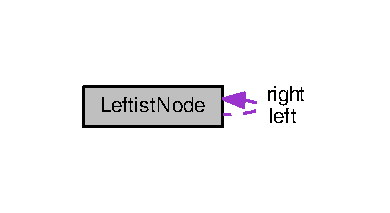
\includegraphics[width=187pt]{classLeftistNode__coll__graph}
\end{center}
\end{figure}
\subsection*{Public Member Functions}
\begin{DoxyCompactItemize}
\item 
\hyperlink{classLeftistNode_a9004469a6ac77c56b47a8a167f17c42f}{Leftist\+Node} (int \&\hyperlink{classLeftistNode_a39afeded6425dbd13bbfd1d9fffb8a95}{element}, \hyperlink{classLeftistNode}{Leftist\+Node} $\ast$lt=N\+U\+LL, \hyperlink{classLeftistNode}{Leftist\+Node} $\ast$rt=N\+U\+LL, int np=0)
\end{DoxyCompactItemize}
\subsection*{Public Attributes}
\begin{DoxyCompactItemize}
\item 
int \hyperlink{classLeftistNode_a39afeded6425dbd13bbfd1d9fffb8a95}{element}
\item 
\hyperlink{classLeftistNode}{Leftist\+Node} $\ast$ \hyperlink{classLeftistNode_a62469c988fc0537dd6682d56f2108d99}{left}
\item 
\hyperlink{classLeftistNode}{Leftist\+Node} $\ast$ \hyperlink{classLeftistNode_aee2ba46112890733b87007103122fc2a}{right}
\item 
int \hyperlink{classLeftistNode_afcd068d744065dc1201d1f738b923447}{npl}
\end{DoxyCompactItemize}


\subsection{Constructor \& Destructor Documentation}
\index{Leftist\+Node@{Leftist\+Node}!Leftist\+Node@{Leftist\+Node}}
\index{Leftist\+Node@{Leftist\+Node}!Leftist\+Node@{Leftist\+Node}}
\subsubsection[{\texorpdfstring{Leftist\+Node(int \&element, Leftist\+Node $\ast$lt=\+N\+U\+L\+L, Leftist\+Node $\ast$rt=\+N\+U\+L\+L, int np=0)}{LeftistNode(int &element, LeftistNode *lt=NULL, LeftistNode *rt=NULL, int np=0)}}]{\setlength{\rightskip}{0pt plus 5cm}Leftist\+Node\+::\+Leftist\+Node (
\begin{DoxyParamCaption}
\item[{int \&}]{element, }
\item[{{\bf Leftist\+Node} $\ast$}]{lt = {\ttfamily NULL}, }
\item[{{\bf Leftist\+Node} $\ast$}]{rt = {\ttfamily NULL}, }
\item[{int}]{np = {\ttfamily 0}}
\end{DoxyParamCaption}
)\hspace{0.3cm}{\ttfamily [inline]}}\hypertarget{classLeftistNode_a9004469a6ac77c56b47a8a167f17c42f}{}\label{classLeftistNode_a9004469a6ac77c56b47a8a167f17c42f}

\begin{DoxyCode}
19         \{
20             this->\hyperlink{classLeftistNode_a39afeded6425dbd13bbfd1d9fffb8a95}{element} = \hyperlink{classLeftistNode_a39afeded6425dbd13bbfd1d9fffb8a95}{element};
21             \hyperlink{classLeftistNode_aee2ba46112890733b87007103122fc2a}{right} = rt;
22             \hyperlink{classLeftistNode_a62469c988fc0537dd6682d56f2108d99}{left} = lt,
23             \hyperlink{classLeftistNode_afcd068d744065dc1201d1f738b923447}{npl} =  np;
24         \}
\end{DoxyCode}


\subsection{Member Data Documentation}
\index{Leftist\+Node@{Leftist\+Node}!element@{element}}
\index{element@{element}!Leftist\+Node@{Leftist\+Node}}
\subsubsection[{\texorpdfstring{element}{element}}]{\setlength{\rightskip}{0pt plus 5cm}int Leftist\+Node\+::element}\hypertarget{classLeftistNode_a39afeded6425dbd13bbfd1d9fffb8a95}{}\label{classLeftistNode_a39afeded6425dbd13bbfd1d9fffb8a95}
\index{Leftist\+Node@{Leftist\+Node}!left@{left}}
\index{left@{left}!Leftist\+Node@{Leftist\+Node}}
\subsubsection[{\texorpdfstring{left}{left}}]{\setlength{\rightskip}{0pt plus 5cm}{\bf Leftist\+Node}$\ast$ Leftist\+Node\+::left}\hypertarget{classLeftistNode_a62469c988fc0537dd6682d56f2108d99}{}\label{classLeftistNode_a62469c988fc0537dd6682d56f2108d99}
\index{Leftist\+Node@{Leftist\+Node}!npl@{npl}}
\index{npl@{npl}!Leftist\+Node@{Leftist\+Node}}
\subsubsection[{\texorpdfstring{npl}{npl}}]{\setlength{\rightskip}{0pt plus 5cm}int Leftist\+Node\+::npl}\hypertarget{classLeftistNode_afcd068d744065dc1201d1f738b923447}{}\label{classLeftistNode_afcd068d744065dc1201d1f738b923447}
\index{Leftist\+Node@{Leftist\+Node}!right@{right}}
\index{right@{right}!Leftist\+Node@{Leftist\+Node}}
\subsubsection[{\texorpdfstring{right}{right}}]{\setlength{\rightskip}{0pt plus 5cm}{\bf Leftist\+Node}$\ast$ Leftist\+Node\+::right}\hypertarget{classLeftistNode_aee2ba46112890733b87007103122fc2a}{}\label{classLeftistNode_aee2ba46112890733b87007103122fc2a}


The documentation for this class was generated from the following file\+:\begin{DoxyCompactItemize}
\item 
\hyperlink{LeftListHeap_8cpp}{Left\+List\+Heap.\+cpp}\end{DoxyCompactItemize}

\chapter{File Documentation}
\hypertarget{LeftListHeap_8cpp}{}\section{Left\+List\+Heap.\+cpp File Reference}
\label{LeftListHeap_8cpp}\index{Left\+List\+Heap.\+cpp@{Left\+List\+Heap.\+cpp}}
{\ttfamily \#include $<$iostream$>$}\\*
{\ttfamily \#include $<$cstdlib$>$}\\*
Include dependency graph for Left\+List\+Heap.\+cpp\+:
\nopagebreak
\begin{figure}[H]
\begin{center}
\leavevmode
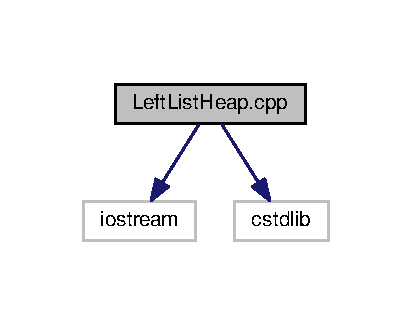
\includegraphics[width=198pt]{LeftListHeap_8cpp__incl}
\end{center}
\end{figure}
\subsection*{Classes}
\begin{DoxyCompactItemize}
\item 
class \hyperlink{classLeftistNode}{Leftist\+Node}
\item 
class \hyperlink{classLeftistHeap}{Leftist\+Heap}
\end{DoxyCompactItemize}
\subsection*{Functions}
\begin{DoxyCompactItemize}
\item 
int \hyperlink{LeftListHeap_8cpp_ae66f6b31b5ad750f1fe042a706a4e3d4}{main} ()
\end{DoxyCompactItemize}


\subsection{Function Documentation}
\index{Left\+List\+Heap.\+cpp@{Left\+List\+Heap.\+cpp}!main@{main}}
\index{main@{main}!Left\+List\+Heap.\+cpp@{Left\+List\+Heap.\+cpp}}
\subsubsection[{\texorpdfstring{main()}{main()}}]{\setlength{\rightskip}{0pt plus 5cm}int main (
\begin{DoxyParamCaption}
{}
\end{DoxyParamCaption}
)}\hypertarget{LeftListHeap_8cpp_ae66f6b31b5ad750f1fe042a706a4e3d4}{}\label{LeftListHeap_8cpp_ae66f6b31b5ad750f1fe042a706a4e3d4}

\begin{DoxyCode}
243 \{
244     \hyperlink{classLeftistHeap}{LeftistHeap} h;
245     \hyperlink{classLeftistHeap}{LeftistHeap} h1;
246     \hyperlink{classLeftistHeap}{LeftistHeap} h2;
247     \textcolor{keywordflow}{for} (\textcolor{keywordtype}{int} i = 0; i < 20; i++)
248     \{
249         \textcolor{keywordflow}{if} (i % 2 == 0)
250         \{
251             h.\hyperlink{classLeftistHeap_a1864cb85655de68ab0813579bd9b9659}{Insert}(i);
252             cout<<\textcolor{stringliteral}{"Element"}<<i<<\textcolor{stringliteral}{" inserted in Heap 1"}<<endl;
253         \}
254         \textcolor{keywordflow}{else}
255         \{
256             h1.\hyperlink{classLeftistHeap_a1864cb85655de68ab0813579bd9b9659}{Insert}(i);
257             cout<<\textcolor{stringliteral}{"Element"}<<i<<\textcolor{stringliteral}{" inserted in Heap 2"}<<endl;
258         \}
259     \}
260     h.\hyperlink{classLeftistHeap_a30c5065cf2bd8c1816d944576f704cc7}{Merge}(h1);
261     h2 = h;
262     \textcolor{keywordflow}{for} (\textcolor{keywordtype}{int} i = 0; i < 20; i++)
263     \{
264         \textcolor{keywordtype}{int} x;
265         h2.\hyperlink{classLeftistHeap_a41ab51a043541d4372fe10cd06561028}{deleteMin}(x);
266         cout<<\textcolor{stringliteral}{"Element "}<<x<<\textcolor{stringliteral}{" Deleted"}<<endl;
267         \textcolor{keywordflow}{if} (h2.\hyperlink{classLeftistHeap_a107b474e1c9f2a15710842d778305ca4}{isEmpty}())
268         \{
269             cout<<\textcolor{stringliteral}{"The Heap is Empty"}<<endl;
270             \textcolor{keywordflow}{break};
271         \}
272     \}
273     \textcolor{keywordflow}{return} 0;
274 \}\end{DoxyCode}


Here is the call graph for this function\+:
\nopagebreak
\begin{figure}[H]
\begin{center}
\leavevmode
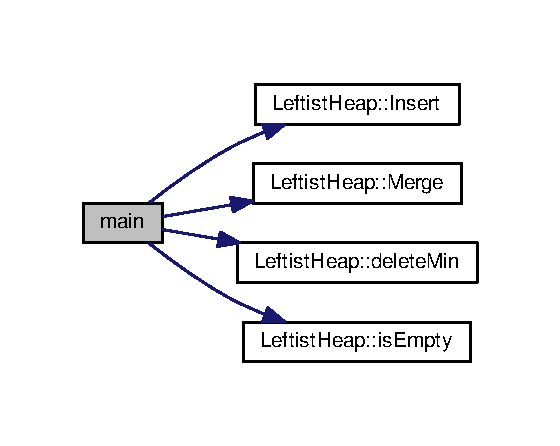
\includegraphics[width=269pt]{LeftListHeap_8cpp_ae66f6b31b5ad750f1fe042a706a4e3d4_cgraph}
\end{center}
\end{figure}



%--- End generated contents ---

% Index
\backmatter
\newpage
\phantomsection
\clearemptydoublepage
\addcontentsline{toc}{chapter}{Index}
\printindex

\end{document}
